\subsubsection{Exercise}

The impact of each input can be measured as: $$\frac{|y_{\text{paired to } u_i}|}{|y_{\text{not-paired}}|}$$

We have the following relation:
\begin{shortitemize}
    \item Input (1):
$$\frac{|y_{1,m}|_\infty}{|y_{2,m}|_\infty} = \frac{.6}{.4} = 1.5 \leq \frac{|y_{2,nm}|_\infty}{|y_{1,nm}|_\infty} = \frac{.7}{.4} = 1.75$$  
    \item Input (2):
$$\frac{|y_{2,m}|_\infty}{|y_{1,m}|_\infty} = \frac{.6}{.3} = 2 \geq \frac{|y_{1,nm}|_\infty}{|y_{2,nm}|_\infty} = \frac{.6}{.4} = 1.5$$ 
\end{shortitemize}

This result can be sum up as:

\begin{center}
\begin{tabular}{|c|cc|}
    \hline
    Desired control & $y_1$ & $y_2$ \\ 
    \hline
    \multirow{2}*{$G_m(s)$} & Act on $u_1$ & Act on $u_2$ \\ 
                & \emph{Stronger} & \emph{Weaker}\\
                & \emph{coupling} & \emph{coupling} \\ 
    \hline
    \multirow{2}*{$G_{nm}(s)$} & Act on $u_2$ & Act on $u_1$ \\
             & \emph{Weaker} & \emph{Stronger}\\
             & \emph{coupling} & \emph{coupling} \\
    \hline
\end{tabular}
\end{center}

\begin{figure}[h!t]
    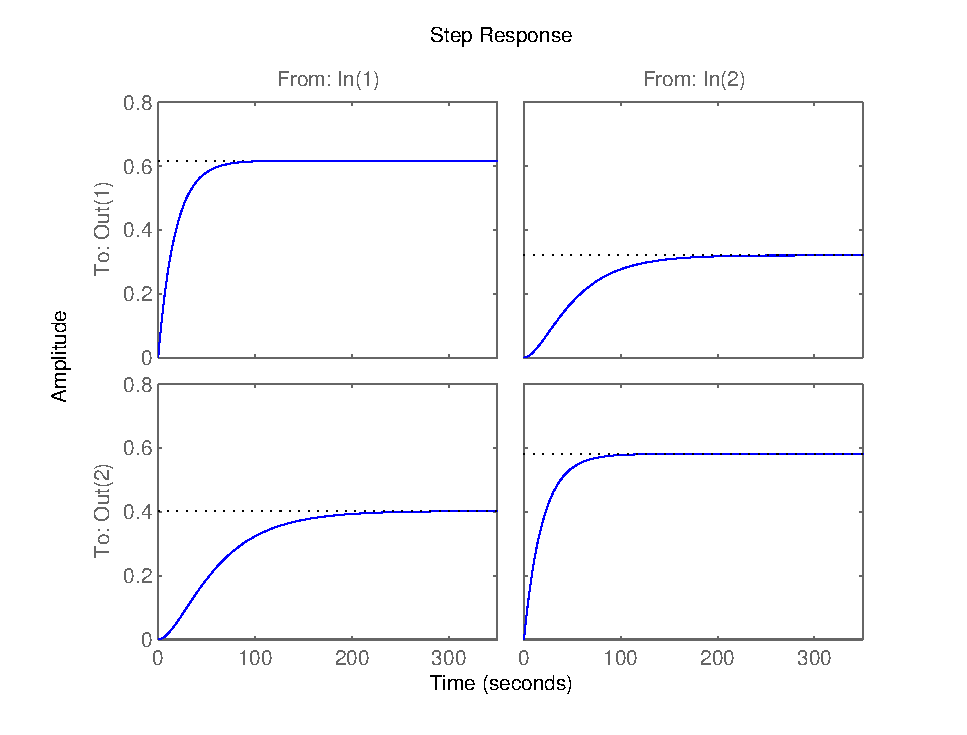
\includegraphics[width=\columnwidth]{fig/step315m}
    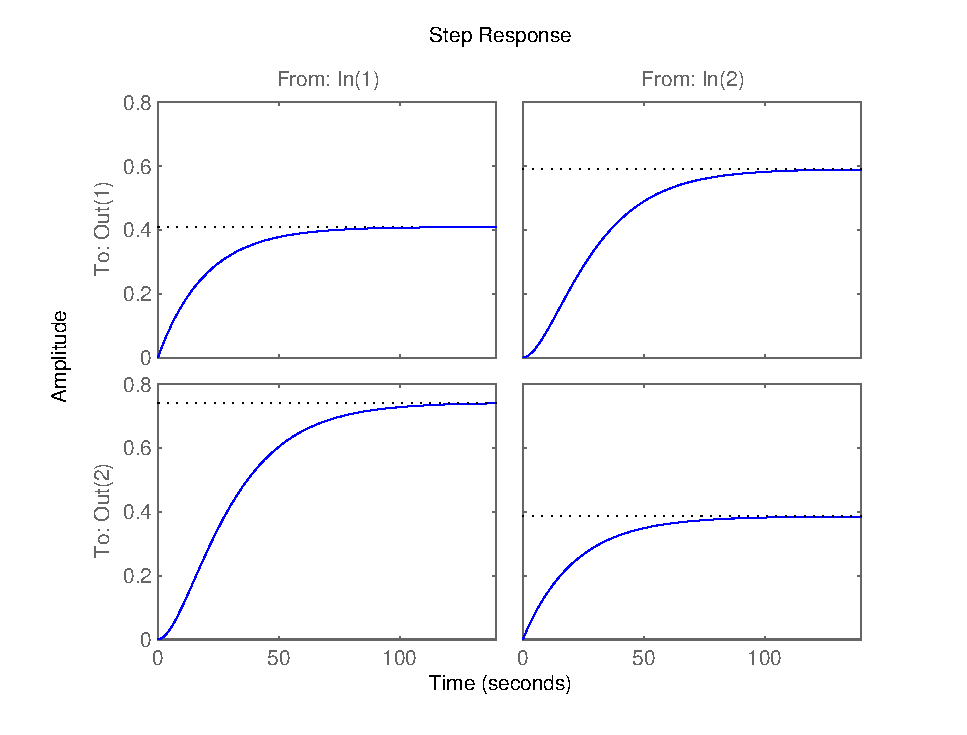
\includegraphics[width=\columnwidth]{fig/step315nm}
    \caption{Step responses of the systems \\ Minimum phase system (top) and non-minimum phase system (bottom)}    
    \label{step315}
\end{figure}
